\documentclass[wd]{isov2}

\usepackage{amsmath}
\usepackage{graphicx}
\usepackage{float}
\usepackage{textcomp}
\usepackage{color}

\let\ifpdf\undefined
\pdfoutput=1
\usepackage[plainpages=false, pdfpagelabels, bookmarksnumbered, hyperindex=true, pdfborder={0 0 0}]{hyperref}
\hypersetup{pdftitle={N1519: Latency Reducing Memory Allocation in the C standard library}, pdfauthor={Niall Douglas}, pdfsubject={ISO/IEC JTC1/SC22/WG14}, pdfkeywords={C1X, N1519}}

\newcommand{\superscript}[1]{\ensuremath{^{\textrm{#1}}}}
\newcommand{\subscript}[1]{\ensuremath{_{\textrm{#1}}}}
\definecolor{changed}{rgb}{0,0.33,0}

\standard{ISO SC22/WG14 -- N1519: Latency Reducing Memory Allocation}
\yearofedition{\hfill [v1.92 Oct 2010]}

\begin{document}

\title{N1519: Latency Reducing Memory Allocation in the C standard library}{\linebreak \large{A minimal change in the dynamic memory allocation API in order to reduce system memory bandwidth usage}}{}
\maxtocdepth{sssclause}

v1.92 14th October 2010

Niall Douglas MBS MA BSc \hfill ned Productions IT Consulting Limited \linebreak
Cork, Ireland \hfill {\url{http://www.nedproductions.biz/}

\small{\begin{itemize}
\item \textbf{Changelog:}
\tiny{\begin{itemize}
\item v1.92 final (14th Oct 2010): Fixed up various typos. Specced the scenario when \texttt{struct mallocation *} is NULL.
\item v1.91 draft 1 (11th Oct 2010): Pre-release to those who have partaken in consultation process so far.
\item v1.00 (8th Sept 2010): First release onto \url{http://mallocv2.wordpress.com/}.
\end{itemize}}
\end{itemize}}

\begin{verbatim}
\end{verbatim}

\begin{foreword}
As is made very clear in Figure \ref{FigMemorySizeVsSpeed}, the past twelve years have seen a 25x linear improvement in RAM access speeds versus a \textbf{250x} \emph{exponential} improvement in RAM capacities. If these trends continue, in 2021 RAM capacity growth will have outpaced growth in its access speed by 3 x 10\superscript{13} times!

Such a mismatch in rates of growth, even if only a fraction of 3 x 10\superscript{13}\footnote{Growth in all things constrained follows a logistic curve whereby the first third is approximately exponential, the second third is approximately linear and the final third is approximately inverse exponential. As a result, the projected mismatch in growth may be anything \emph{up to} 3 x 10\superscript{13} but one cannot yet say for sure by how much.}, has \textbf{profound} long term consequences for computer software design which presently overwhelmingly assumes that RAM capacity -- not its speed of access -- is that which is scarce. Virtual memory, as described in Denning's classic 1970 paper \bref{denning1970virtual}, was developed as a system which sacrifices access speed (especially first time page access latency) for the ability to allow software to be written as if available RAM capacity is higher than it really is. Unfortunately, in the next decade it will be \emph{access speeds} which will be far more scarce than capacity.

\begin{figure}[h]
  \centering
    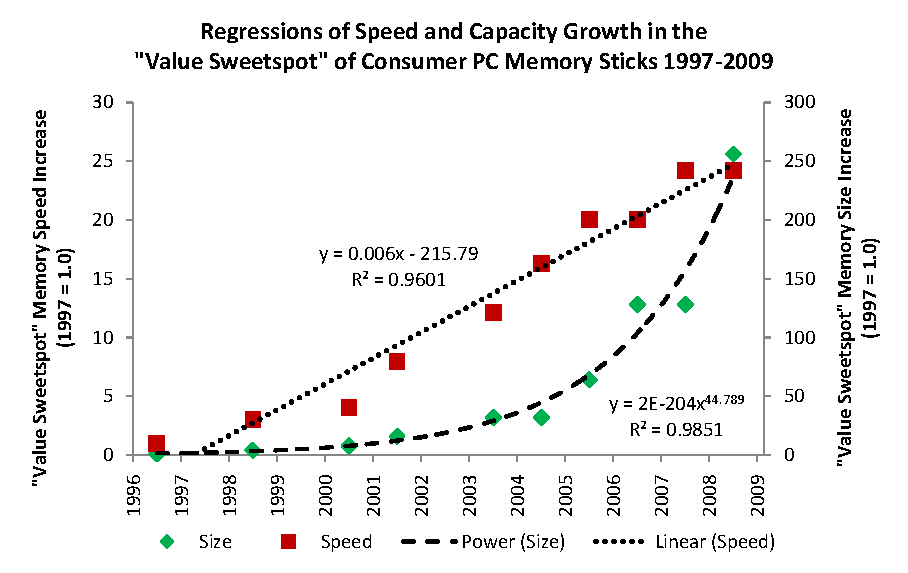
\includegraphics{MemorySizeVsSpeed}
  \caption{A plot of the relative growths since 1997 of random access memory (RAM) speeds and sizes for the best value (in terms of Mb/US\$) memory sticks then available on the US consumer market from 1997 - 2009, with speed depicted by squares on the left hand axis and with size depicted by diamonds on the right hand axis. The dotted line shows the best fit regression for speed which is linear, and the dashed line shows the best fit for size which is a power regression. Note how that during this period memory capacity outgrew memory speed by a factor of ten. Sources: \bref{jcmit2010} \bref{wiki2010}.}
  \label{FigMemorySizeVsSpeed}
\end{figure}

The ISO C memory allocation API (\texttt{malloc()}, \texttt{realloc()}, \texttt{free()} et al) is used by many languages and systems far outside just C: the programming languages of C++, PHP, Python, Perl and Ruby are among the best known languages to also use the C memory allocator. Its design, which predates even the general availability of virtual memory, was crystallised in the Seventh Edition of Unix right back in 1979 (see \url{http://cm.bell-labs.com/7thEdMan/v7vol1.pdf}, page 297) and has been unchanged for decades. It has no concept of block alignment (useful for stream and vector unit computation), no concept of address space reservation (useful for creating space into which arrays can be extended without copy or move construction), no concept of speculative (i.e. non-moving) block resize attempts, no concept of batch operations nor any concept of providing execution context awareness to the memory allocator such that non-constant time operations can be avoided in latency sensitive situations such as interrupt handlers. All of these limitations contribute significant and unnecessary additions to memory bandwidth utilisation via unnecessary VM page committal and use of atomic locking, as well as excessive branchiness in the logic executed by the CPU and therefore to average access latencies across the entire system. This translates into less scalable performance especially in a symmetric multiprocessing configurations, as well as to increased electricity consumption due to being unable to prevent the duplication of work performed.

Obviously, in time, the whole concept of what virtual memory is and how it is implemented will need to be addressed, but we are not at that point yet. However, given that it can take up to a decade for ISO standard changes to become generally available to programmers, surely \textbf{now} is the time to introduce the most obvious and least controversial memory bandwidth utilisation and latency reducing improvements?

I am certainly not the person with sufficient expertise to propose such wide ranging changes to an entire programming language. My area of expertise is relatively small: I am the author of a reasonably popular third-party memory allocator called nedmalloc \bref{nedmalloc}, and for many years I have felt that the C memory allocation API really needed a few small tweaks to help its users make better use of it. To that end, during the summer of 2010 I had informal discussions with a number of people as to what form these changes ought to take. In the Autumn of 2010, I launched a single purpose website at \url{http://mallocv2.wordpress.com/} containing an early draft of the text herein with a commenting system and announced it as widely as I could, and indeed many useful comments did ensue. The standards text changes proposed in this document are the result of my best attempts to coalesce the many suggestions, ideas and thoughts which have been gathered over these recent months from all the parties involved.

Choosing what to include, or more accurately, what to \emph{exclude} from this change proposal has not been easy. Given the luke warm to cold reception given by the ISO committees to previous attempts to change the memory allocation API in C++\footnote{Specifically, the ISO/IEC JTC1/SC22/WG21 papers N1850, N2045 and N2271.}, I felt that if this proposal has any chance whatsoever of being accepted then it needs to be absolutely as \textbf{small} as possible. To that end, I have specifically removed as much of what \emph{could} and perhaps ought to be improved as possible, and hopefully as a result leaving the minimum needed which \emph{needs} to be changed in order to reduce system utilisation of memory bandwidth. As a result, implementation time is very quick: approximately \textbf{fifteen man-hours} was required to modify a copy of dlmalloc \bref{dlmalloc}, including testing, for Microsoft Windows and POSIX Linux using standard system APIs. There is no reason to believe that any changes introduced by this proposal would have any adverse effect on any architecture for which ISO C is supported.

My thanks go to all those who participated in these discussions. In particular, I would like to thank Doug Lea for his unwavering advice, support and help throughout the past five years; Jason Evans (author of jemalloc, the allocator used by Mozilla Firefox and the BSD standard C library implementation) for a very detailed and comprehensive response to this proposal; Peter Buhr for his detailed thoughts and discussions concerning whether alignment should be a sticky property of allocated blocks; and both Jeffrey Hellrung and Jeffrey Yasskin for their long and detailed comments and ideas on the mallocv2 single purpose consultative website. I would also like to thank David Dice and John Benito, as well as David Keaton, Blaine Garst, Thomas Plum and Larry Jones for their useful feedback. Lastly I would like to thank those on the Usenet discussion group \texttt{comp.std.c} for their responses -- if I knew your real names I would give them here!

\begin{flushleft}
Niall Douglas\linebreak
11th October 2010\linebreak
Cork, Ireland.
\end{flushleft}
\end{foreword}

\begin{introduction}
Before I detail the specific proposed changes to N1494, the C1X working draft text, I thought it appropriate that a quick overview is given of the design choices made during the development of this proposal and why these were made. Given the severe importance of the memory allocator API far outside the C programming language, I think it important to show what consideration was given to what and why.

Features of this proposal:
\begin{enumerate}
\item A two tier memory allocation API composed of the simple, easy to use API and the complex, powerful API. In all cases the simple API calls the complex API with predefined parameters (and example implementations are supplied in this proposal text).
\item As has always been the case in C, any block allocated by any of the memory management functions is interchangeable with any other block allocated by those functions. In other words, you can always \texttt{free()} or \texttt{realloc()} any allocated block no matter how so allocated via the standard API. This guarantee greatly simplifies block management, especially where one cannot use templated types to enforce pointer management traits as one would in C++.
\item The complex API is fundamentally a batch operator permitting \emph{very} significant performance increases. Three forms are given which differ only in the amount of data they consume and output. Care was taken to ensure that a single implementation for all three complex APIs can be written, and the compiler's optimizer is left with the task of reducing that single implementation down to an optimal configuration for each call. Care was also taken to segment the cache lines between the data used by each operation such that an OpenMP based parallel execution would perform optimally.
\item The ability to obtain the \emph{actual} size allocated which may in some circumstances be much larger than the size requested.
\item The ability to resize an aligned block while maintaining alignment. This feature is very useful for expanding arrays of sixteen byte aligned vectors such as is required by SSE and AVX based CPU vector extensions.
\item The ability to attempt the resizing of a block which returns failure if the block cannot be resized without relocating it. This feature is \emph{particularly} useful for object orientated languages such as C++.
\item The ability to reserve address space which allows \texttt{realloc()} to expand an allocation into the reserved region without relocating it. This feature is absolutely essential for systems not providing a fault driven page allocation system\footnote{Note that I have a forthcoming academic paper detailing the performance and scalability gains enabled by outsourcing the kernel memory page management system into user space by making use of the hardware virtualisation of the CPU's Memory Management Unit. Under such a system, almost the entire process of memory management within each process can be made independent from all other processes, however one of the consequences is that committing memory really does commit a real page of memory rather than a placeholder which is later made real when first accessed by the CPU. Therefore, over-committing memory through asking for a block size far larger than is actually needed -- which is currently how address reservation is implemented -- would waste significant amounts of real physical RAM.}, and even for traditional paged virtual memory systems it significantly helps to reduce the amount of memory copying and memory zeroing performed throughout the system i.e. a great reduction in memory bandwidth utilisation\footnote{For applications which perform a lot of large allocations and frees -- e.g. the GNU C++ compiler -- the performance gain from this alone can be up to 10\% already today. As memory capacity utilisation increases, this benefit will increase.}.
\item The ability to request that any non-essential processing (such as segment coalescing) is not performed during a particular call. This feature is very useful for usage of the memory allocator during time critical semi-periodic routines such as interrupt handlers.
\item A formal interface allowing third party additions to functionality via the \texttt{flags} parameter. This feature is useful for enabling most of the features which were considered but not included (listed below) as well as testing experimental allocators.
\item For the purposes of compatibility with POSIX, the batch operators can optionally output the \texttt{errno} result for each operation into an array. This avoids having to run through a thread local variable, and is therefore very fast.
\end{enumerate}

~ \linebreak
Features which were considered but NOT included:
\begin{enumerate}
\item The ability to traverse and query memory to discover its state and use context e.g. in which allocated block is an address located? Is a location in reserved, allocated or free memory? To which execution binary does this location belong? And so on.
\begin{description}
\item[Rationale] While highly desirable due to its usefulness in many scenarios such as working out from where to load translations of user interface text, I could not see how to standardise such a facility across all platforms including those of the near future. Additionally, the assumptions required about the facilities provided by the host operating system are very high and too high in my opinion for an ISO standard.
\end{description}
\item The ability to specify the block's size during a \texttt{free()} operation, thus saving the need to look up a block's size and/or the need to store the block's size.
\begin{description}
\item[Rationale] As much as memory allocation specialists would love this feature, it introduces significant inter-operability problems between different blocks allocated via different means. It also introduces problems with security and potentially malevolent usage, and indeed the overheads introduced by ensuring that the size given is feasible would be far slower than not having it at all.
\end{description}
\item Backwards block resizing i.e. where the pointer to the block is moved backwards in memory into a preceding region of free space. This is useful in a wide range of algorithms such as deque and various forms of buffering as well as helping to reduce memory fragmentation and increase cache locality.
\begin{description}
\item[Rationale] Given how infrequently this feature would be used and the potential consequences upon internal implementation for some types of allocator, I felt that such a feature ought not to be standardised. There is no reason why third-party support for this feature cannot be added via the \texttt{flags} parameter.
\end{description}
\item Iterator based rather than array based batch operators. This is useful as it avoids having to preallocate scratch space as well as being much more amenable to many kinds of idiomatic usage, especially in C++.
\begin{description}
\item[Rationale] My difficulty with this idea is how to implement it safely and efficiently in C while allowing the use of OpenMP to parallelise the batch operation. I came to the conclusion that array based batch operations are much easier, and besides either variable length arrays or the magic stack allocation function \texttt{alloca()} is available on almost all platforms nowadays.
\end{description}
\item Segregated allocation pools. This is a very useful feature allowing a large range of security and performance improvements to be made. Its exclusion will no doubt be one of the most controversial.
\begin{description}
\item[Rationale] My difficulty in standardising this was to encapsulate all possible use scenarios. For example, an allocation pool which exists in cryptographically secure or transactional memory is very feasible, as are allocation pools which exist on non-local NUMA nodes. I am sure that these will become standardised one day, but I don't think that time is now.
\end{description}
\item Node vs. Array allocation, where the latter is a form of stack based allocator useful for temporary allocations. This class of allocation strategy serves as a middle-man between stack based and full heap based allocation, and due to its speed it is one of the most common reasons to employ a `non-standard' memory allocation technique (Berger et al, 2002) \bref{berger2002reconsidering}.
\begin{description}
\item[Rationale] My difficulty here is that this type of allocator is essentially an ``increment the pointer" system which offers no protection against memory corruption and malevolent or erroneous usage. Without a proper deployment of ``anti-stack smashing" measures -- which implies that the memory used for such allocations must come from a separate execution bit disabled source -- it would reopen many of the security problems in C based code only very recently quashed. Also, pointers returned from the array allocator could not be interchanged with pointers returned from the node allocator as the former lack the metadata (i.e. the header and footer of the block) required to allow it unless magic segment headers are employed\footnote{Magic segment headers work by aligning the address of segments to round multiples, so for example one might round segments to 2Mb (a `huge page' on x64) boundaries. One can then always find the `owning' segment for a block by masking out the bottom 2Mb of bits and checking for a magic value at that location.}.
\end{description}
\item Thread local pool allocation. This is a feature used by modern Java implementations to allow the allocation and deallocation of memory in tens of CPU cycles rather than the hundreds (or thousands) of CPU cycles required by even the simplest \texttt{malloc()} invocation.
\begin{description}
\item[Rationale] This looks like a very desirable feature on paper, especially given that Java's memory allocation performance is several orders faster than that of C's. However, Java's runtime has exclusive access to its environment which allows it to make assumptions about how memory will be used. In fact, this feature is a form of an ``increment the pointer" allocator with all its attendent problems, so all the problems there apply here too. There is no reason however why third-party support for this feature cannot be added via the \texttt{flags} parameter.
\end{description}
\end{enumerate}

\end{introduction}

\normrefsclause
\normrefbp{proposal}
\begin{nreferences}
\isref{ISO/IEC 9899}{Programming Language C}
\disref{ -- N1494}{{Next revision of C standard, `C1X', \url{http://www.open-std.org/jtc1/sc22/wg14/www/docs/n1494.pdf}}}
\end{nreferences}
The remainder of this document is based on the \textbf{June 25th 2010} edition of N1494.

\scopeclause
\begin{inscope}{proposal}
\item Section 7.5.2 (Errors \texttt{<errno.h>}) in ISO/IEC 9899:N1494.
\item The preamble of Section 7.22 (General utiltiies \texttt{<stdlib.h>}) in ISO/IEC 9899:N1494.
\item Section 7.22.3 (Memory Management functions) in ISO/IEC 9899:N1494.
\end{inscope}

\clause{The proposed changes to the C programming language standard}
Dark green highlighting has been used to distinguish the additions to the original text.
\setsecnumdepth{clause}

\sclause{7.5 Errors \texttt{<errno.h>}}
\begin{enumerate}
\renewcommand{\theenumi}{\arabic{enumi}}
\item The header \texttt{<errno.h>} defines several macros, all relating to the reporting of error conditions.
\item The macros are

\texttt{EDOM\linebreak
EILSEQ\linebreak
\textcolor{changed}{ENOMEM}\linebreak
\textcolor{changed}{ENOSPC}\linebreak
ERANGE}

which expand to integer constant expressions with type \texttt{int}, distinct positive values, and which are suitable for use in \texttt{\#if} preprocessing directives; and

\texttt{errno}

which expands to a modifiable lvalue that has type \texttt{int} and thread local storage duration, the value of which is set to a positive error number by several library functions. If a macro definition is suppressed in order to access an actual object, or a program defines an identifier with the name \texttt{errno}, the behavior is undefined.
\end{enumerate}

\sclause{7.22 General utilities \texttt{<stdlib.h>}}
\begin{enumerate}
\renewcommand{\theenumi}{\arabic{enumi}}
\item The header \texttt{<stdlib.h>} declares five types\textcolor{changed}{, two structures} and several functions of general utility, and defines several macros.
\item The types declared are \texttt{size\_t} and \texttt{wchar\_t} (both described in 7.19),

\texttt{div\_t}

which is a structure type that is the type of the value returned by the \texttt{div} function,

\texttt{ldiv\_t}

which is a structure type that is the type of the value returned by the \texttt{ldiv} function, and

\texttt{lldiv\_t}

which is a structure type that is the type of the value returned by the \texttt{lldiv} function.
\color{changed}
\item The structures declared are
\begin{verbatim}
#ifndef MALLOCATION2_DEFINED
#define MALLOCATION2_DEFINED
struct mallocation2 {
    void *ptr;
    size_t size;
};
#endif
\end{verbatim}
which is used by the \texttt{batch\_alloc2} function; and
\begin{verbatim}
#ifndef MALLOCATION5_DEFINED
#define MALLOCATION5_DEFINED
struct mallocation5 {
    void *ptr;
    size_t size;
    size_t alignment;
    size_t reserve;
    uintmax_t flags;
};
#endif
\end{verbatim}
which is used by the \texttt{batch\_alloc5} function.
\color{black}
\item The macros defined are \texttt{NULL} (described in 7.19);

\texttt{EXIT\_FAILURE}

and

\texttt{EXIT\_SUCCESS}

which expand to integer constant expressions that can be used as the argument to the exit function to return unsuccessful or successful termination status, respectively, to the host environment;

\texttt{RAND\_MAX}

which expands to an integer constant expression that is the maximum value returned by the rand function; and

\texttt{MB\_CUR\_MAX}

which expands to a positive integer expression with type \texttt{size\_t} that is the maximum number of bytes in a multibyte character for the extended character set specified by the current locale (category \texttt{LC\_CTYPE}), which is never greater than \texttt{MB\_LEN\_MAX}\color{changed};

\texttt{M2\_ZERO\_MEMORY}

which is a single set bit in an integer which when set in the \texttt{flags} parameter of one of the \texttt{batch\_alloc*} functions requests the memory allocator to return any newly allocated space initialized to all bits zero;

\texttt{M2\_PREVENT\_MOVE}

which is a single set bit in an integer which when set in the \texttt{flags} parameter of one of the \texttt{batch\_alloc*} functions inhibits the address relocation of an object being resized by the memory allocator;

\texttt{M2\_CONSTANT\_TIME}

which is a single set bit in an integer which when set in the \texttt{flags} parameter of one of the \texttt{batch\_alloc*} functions requests that the memory allocator avoid any non-essential (e.g. housekeeping) operations (which may take an unpredictable length of time) during this particular operation;

\texttt{M2\_RESERVE\_IS\_MULT}

which is a single set bit in an integer which when set in the \texttt{flags} parameter of one of the \texttt{batch\_alloc*} functions causes the memory allocator to multiply the reservation size by the usable size of the block at the time of this particular operation before usage;

\texttt{M2\_BATCH\_IS\_ALL\_ALLOC}

which is a single set bit in an integer which when set in the \texttt{flags} parameter of one of the \texttt{batch\_alloc*} functions causes the memory allocator to assume that all the operations in this batch are allocations of new objects (i.e. no resizing, no modifications, no deallocations);

\texttt{M2\_BATCH\_IS\_ALL\_REALLOC}

which is a single set bit in an integer which when set in the \texttt{flags} parameter of one of the \texttt{batch\_alloc*} functions causes the memory allocator to assume that all the operations in this batch are modifications of existing objects (i.e. no new allocations, no deallocations);

\texttt{M2\_BATCH\_IS\_ALL\_FREE}

which is a single set bit in an integer which when set in the \texttt{flags} parameter of one of the \texttt{batch\_alloc*} functions causes the memory allocator to assume that all the operations in this batch are deallocations of existing objects (i.e. no new allocations, no resizing, no modifications);

\texttt{M2\_USERFLAGS\_FIRST}

which is the first available bit set aside for use by allocator extensions in the \texttt{flags} parameter of one of the \texttt{batch\_alloc*} functions; and

\texttt{M2\_USERFLAGS\_LAST}

which is the last available bit set aside for use by allocator extensions in the \texttt{flags} parameter of one of the \texttt{batch\_alloc*} functions\footnote{For example, these might be \texttt{\#define M2\_USERFLAGS\_FIRST (1<<16)} and \texttt{\#define M2\_USERFLAGS\_LAST (1<<31)}, so allocator extensions can in this situation use the bits denoted by the set bits in the mask \texttt{0xFFFF0000}.}.
\end{enumerate}

\ssclause{7.22.3 Memory management functions}
\begin{enumerate}
\renewcommand{\theenumi}{\arabic{enumi}}
\item The order and contiguity of storage allocated by successive calls to the \texttt{aligned\_alloc}, \textcolor{changed}{\texttt{batch\_alloc*}}, \texttt{calloc}, \texttt{malloc}, and \texttt{realloc} functions is unspecified. The pointer returned if the allocation succeeds is suitably aligned so that it may be assigned to a pointer to any type of object with a fundamental alignment requirement and then used to access such an object or an array of such objects in the space allocated (until the space is explicitly deallocated). The lifetime of an allocated object extends from the allocation until the deallocation. Each such allocation shall yield a pointer to an object disjoint from any other object. The pointer returned points to the start (lowest byte address) of the allocated space. If the space cannot be allocated \textcolor{changed}{according to the parameters supplied}, a null pointer is returned. If the size of the space requested is zero, the behavior is implementation-defined: either a null pointer is returned, or the behavior is as if the size were some nonzero value, except that the returned pointer shall not be used to access an object.
\end{enumerate}

\sssclause{7.22.3.1 The aligned\_alloc function}
\ssssclause{Synopsis}
\begin{enumerate}
\renewcommand{\theenumi}{\arabic{enumi}}
\item \texttt{\#include <stdlib.h>\linebreak
void *aligned\_alloc(size\_t alignment, size\_t size);}
\ssssclause{Description}
\item The \texttt{aligned\_alloc} function allocates space for an object whose alignment is specified by \texttt{alignment}, whose size is specified by \texttt{size}, and whose value is indeterminate. The value of \texttt{alignment} shall be a valid alignment supported by the implementation and the value of \texttt{size} shall be an integral multiple of \texttt{alignment}.
\color{changed}
\item The effects of the \texttt{aligned\_alloc} function shall be equivalent to:
\begin{verbatim}
void *aligned_alloc(size_t alignment, size_t size)
{
    void *mem=0;
    size_t count=1;
    /* Optional */ if(0==size) size=1;
    batch_alloc1(NULL, &mem, &count, &size, alignment, 0, 0);
    return count ? mem : NULL;
}
\end{verbatim}
\color{black}
\ssssclause{Returns}
\item The \texttt{aligned\_alloc} function returns either a null pointer or a pointer to the allocated space.
\end{enumerate}

\color{changed}
\sssclause{7.22.3.2 The aligned\_realloc function}
\ssssclause{Synopsis}
\begin{enumerate}
\renewcommand{\theenumi}{\arabic{enumi}}
\item \texttt{\#include <stdlib.h>\linebreak
void *aligned\_realloc(void *ptr, size\_t alignment, size\_t size);}
\ssssclause{Description}
\item The \texttt{aligned\_realloc} function deallocates the old object pointed to by \texttt{ptr} and returns a pointer to a new object whose alignment is specified by \texttt{alignment} and whose size is specified by \texttt{size}. The contents of the new object shall be the same as that of the old object prior to deallocation, up to the lesser of the new and old sizes. Any bytes in the new object beyond the size of the old object have indeterminate values.
\item If \texttt{ptr} is a null pointer, the \texttt{aligned\_realloc} function behaves like the \texttt{aligned\_malloc} function for the specified alignment and size. Otherwise, if \texttt{ptr} does not match a pointer earlier returned by a memory management function, or if the space has been deallocated by a call to a memory management function, the behavior is undefined. If memory for the new object cannot be allocated, the old object is not deallocated and its value is unchanged.
\color{changed}
\item The effects of the \texttt{aligned\_realloc} function shall be equivalent to:
\begin{verbatim}
void *aligned_realloc(void *ptr, size_t alignment, size_t size)
{
    size_t count=1;
    batch_alloc1(NULL, &ptr, &count, &size, alignment, 0, 0);
    return count ? ptr : NULL;
}
\end{verbatim}
\ssssclause{Returns}
\item The \texttt{aligned\_realloc} function returns a pointer to the new object (which may have the same value as a pointer to the old object), or a null pointer if the new object could not be allocated.
\end{enumerate}
\color{black}

\color{changed}
\sssclause{7.22.3.3 The batch\_alloc1 function}
\ssssclause{Synopsis}
\begin{enumerate}
\renewcommand{\theenumi}{\arabic{enumi}}
\item \begin{verbatim}
#include <stdlib.h>
void **batch_alloc1(int *errnos, void **ptrs, size_t *restrict count,
    size_t *restrict size, size_t alignment, size_t reserve, uintmax_t flags);
\end{verbatim}
\ssssclause{Description}
\item The \texttt{batch\_alloc1} function performs a series of up to \texttt{(*count)} allocations or reallocations of objects each of which is sized to no less than \texttt{(*size)}, or if \texttt{size} is NULL or \texttt{(*size)} is zero then it performs a series of up to \texttt{(*count)} deallocations of objects.
\item Firstly, if \texttt{(*size)} is non-zero, the value of \texttt{(*size)} is modified to be the eventual usable space for each allocation\footnote{In other words, the allocator rounds the size up to whatever its nearest internal granularity is that satisfies the requirements established by the parameters on entry.}, taking account of any non-zero value of \texttt{alignment} if necessary. Secondly, if \texttt{ptrs} is zero, a zero bits filled object sufficient to store a \texttt{(*count)} member array of \texttt{void *} is made and returned on exit (see Returns below) after the completion of the batch operation (in this situation, for obvious reasons only a batch allocation of same sized objects can be performed, though if \texttt{size} is NULL or \texttt{(*size)} is zero then a zero filled array is still returned).
\item Then, for each member of the array \texttt{ptrs[n]} where \texttt{0 $\le$ n $<$ (*count)} (which may be implemented sequentially or in parallel):
\begin{enumerate}
\renewcommand{\theenumii}{\alph{enumii}}
\item If \texttt{size} is NULL or \texttt{(*size)} is zero, and \texttt{ptrs[n]} is zero, no action occurs. This occurrance is considered as always successful for the purposes of calculating \texttt{(*count)} on exit (see Returns below), and if \texttt{errnos} is not NULL then \texttt{errnos[n]} is set to zero.

\item If \texttt{size} is NULL or \texttt{(*size)} is zero, and \texttt{ptrs[n]} is non-zero, the space pointed to by \texttt{ptrs[n]} is deallocated, that is, made available for further allocation. If the pointer to the space does not match a pointer earlier returned by a memory management function, or if the space has been deallocated by a call to a memory management function, the behavior is undefined.

If the deallocation is successful, \texttt{ptrs[n]} is set to zero and if \texttt{errnos} is not NULL, then \texttt{errnos[n]} is also set to zero. If the deallocation is not successful, \texttt{ptrs[n]} is not modified and if \texttt{errnos} is not NULL, then \texttt{errnos[n]} is set to an implementation-dependent value conforming with the requirements of Section 7.5 (Errors \texttt{<errno.h>}).

\item If \texttt{(*size)} is non-zero and \texttt{ptrs[n]} is zero, space is allocated for an object whose alignment is specified by \texttt{alignment} if non-zero, whose size is specified by \texttt{(*size)}, and whose value is indeterminate unless \texttt{flags} contains the flag \texttt{M2\_ZERO\_MEMORY}, whereupon the space shall be initialized to all bits zero. If \texttt{alignment} is non-zero, it shall be a valid alignment supported by the implementation.

If the allocation is successful, \texttt{ptrs[n]} is set to point at the allocated space and if \texttt{errnos} is not NULL, then \texttt{errnos[n]} is also set to zero. If the allocation is not successful and if \texttt{errnos} is not NULL, then \texttt{errnos[n]} is set to one of:
\begin{enumerate}
\item \texttt{ENOMEM} in the situation that the system has insufficient free memory to satisfy the allocation of the object.
\item Otherwise, an implementation-dependent value conforming with the requirements of Section 7.5 (Errors \texttt{<errno.h>}).
\end{enumerate}

\item If \texttt{(*size)} is non-zero and \texttt{ptrs[n]} is non-zero, the properties of the space pointed to by \texttt{ptrs[n]} is modified such that its alignment is at least the value of \texttt{alignment} if non-zero and its usable size is at least the value of \texttt{(*size)}. If the new usable size of the object is greater than the old usable size of the object, the additional bytes beyond the old usable size of the object have interdeterminate values unless \texttt{flags} contains the flag \texttt{M2\_ZERO\_MEMORY}, whereupon the additional bytes shall be initialized to all bits zero. If \texttt{flags} does not contain the flag \texttt{M2\_PREVENT\_MOVE}, the space containing the contents of the object may be relocated to a location with sufficient free space after the object such that the request can be satisfied -- in the event of such a relocation, the contents of \texttt{ptrs[n]} shall be updated to point at the new object storage.

If the modification is successful and if \texttt{errnos} is not NULL, then \texttt{errnos[n]} is also set to zero. If the modification is not successful and if \texttt{errnos} is not NULL, then \texttt{errnos[n]} is set to one of:
\begin{enumerate}
\renewcommand{\theenumii}{\alph{enumii}}
\item \texttt{ENOMEM} in the situation that the system has insufficient free memory to satisfy the expansion of the size of the object.
\item \texttt{ENOSPC} in the situation that the flag \texttt{M2\_PREVENT\_MOVE} was specified and there is insufficient free space existing after the existing object to satisfy the expansion of the size of the object or the alignment of the existing object is not sufficient to match \texttt{alignment}.
\item Otherwise, an implementation-dependent value conforming with the requirements of Section 7.5 (Errors \texttt{<errno.h>}).
\end{enumerate}
\end{enumerate}
\item If the value of \texttt{reserve} is non-zero, the allocator \emph{may} set aside an additional space of at least $($\texttt{reserve} $-$ \texttt{(*size)}$)$ bytes after the usable space occupied by the object such that subsequent expansions of the size of the object up to at least \texttt{reserve} bytes will try to not cause the relocation of the storage of the object. The value of this parameter is treated as a hint of intended use by the application to the allocator\footnote{In particular, 8-bit, 16-bit and 32-bit architectures have limited available address space and so implementations may choose to completely ignore the value of this parameter on the basis that observing it may cause free address space to become exhausted before free physical memory. In addition, present architectures and operating system designs only show a major benefit when object sizes are relatively large (in the order of a few hundred thousand bytes) so allocators may choose to honor this value only with larger object sizes.}, so implementations are free to ignore the value of this parameter in some or all situations or configurations. If \texttt{flags} contains the flag \texttt{M2\_RESERVE\_IS\_MULT}, the value specified by \texttt{reserve} is multiplied by the value of \texttt{(*size)} before use.
\item If the flag \texttt{M2\_BATCH\_IS\_ALL\_ALLOC} has been specified in \texttt{flags}, then all members of \texttt{ptrs[n]} shall be zero on entry or else undefined behavior shall result.
\item If either of the flags \texttt{M2\_BATCH\_IS\_ALL\_REALLOC} or \texttt{M2\_BATCH\_IS\_ALL\_FREE} has been specified in \texttt{flags}, then all members of \texttt{ptrs[n]} shall be non-zero on entry and shall point at a valid space previously returned by a memory management function or else undefined behavior shall result.
\item If the flag \texttt{M2\_BATCH\_IS\_ALL\_FREE} has been specified in \texttt{flags}, then \texttt{size} shall be NULL or \texttt{(*size)} shall be zero or else undefined behavior shall result.
\item The effects of the \texttt{batch\_alloc1} function shall be equivalent to:

\begin{verbatim}
void **batch_alloc1(int *errnos, void **ptrs, size_t *restrict count,
    size_t *restrict size, size_t alignment, size_t reserve, uintmax_t flags)
{
    size_t n, maxn=*count;
    /* Note that some implementations use malloc for variable length
       arrays: this may induce recursion. */
    struct mallocation5 mdata[maxn], *mdataptrs[maxn];
    if(!ptrs && !(ptrs=(void **) calloc(maxn, sizeof(void *))))
    {
        *count=0;
        return NULL;
    }
    for(n=0; n<maxn; n++)
    {
        mdataptrs[n]=mdata+n;
        mdata[n].ptr=ptrs[n];
        mdata[n].size=size ? *size : 0;
        mdata[n].alignment=alignment;
        mdata[n].reserve=reserve;
        mdata[n].flags=flags;
    }
    batch_alloc5(errnos, mdataptrs, count);
    if(size) *size=(size_t)-1;
    for(n=0; n<maxn; n++)
    {
        ptrs[n]=mdata[n].ptr;
        if(size && mdata[n].size<*size) *size=mdata[n].size;
    }
    return ptrs;
}
\end{verbatim}
\ssssclause{Returns}
\item The \texttt{batch\_alloc1} function returns the value of \texttt{ptrs} if it was non-zero on entry. If \texttt{ptrs} was zero on entry, an object sufficient to store a \texttt{(*count)} member array of \texttt{void *} is allocated and returned -- in this situation, the returned pointer must be freed using the \texttt{free} function when its contents are no longer needed. If there was insufficient free memory to allocate the object containing the array of \texttt{void *}, a null pointer is returned and \texttt{(*count)} is set to zero.
\item The \texttt{batch\_alloc1} function sets the value of \texttt{(*size)} to the smallest usable size of any object allocated during the batch operation.
\item The \texttt{batch\_alloc1} function sets the value of \texttt{(*count)} to the number of successful operations executed during the batch operation.
\end{enumerate}

\sssclause{7.22.3.4 The batch\_alloc2 function}
\ssssclause{Synopsis}
\begin{enumerate}
\renewcommand{\theenumi}{\arabic{enumi}}
\item \begin{verbatim}
#include <stdlib.h>
_Bool batch_alloc2(int *errnos, struct mallocation2 **restrict mdataptrs,
   size_t *restrict count, size_t alignment, size_t reserve, uintmax_t flags);
\end{verbatim}
\ssssclause{Description}
\item The \texttt{batch\_alloc2} function performs a series of up to \texttt{(*count)} allocations, reallocations or deallocations of objects.
\item For each member of the array \texttt{mdataptrs[n]} where \texttt{0 $\le$ n $<$ (*count)} (which may be implemented sequentially or in parallel):
\begin{enumerate}
\renewcommand{\theenumii}{\alph{enumii}}
\item If \texttt{mdataptrs[n]} is NULL, or \texttt{mdataptrs[n]->size} is zero and \texttt{mdataptrs[n]->ptr} is zero, no action occurs. This occurrance is considered as always successful for the purposes of calculating \texttt{(*count)} on exit (see Returns below), and if \texttt{errnos} is not NULL then \texttt{errnos[n]} is set to zero.

\item If \texttt{mdataptrs[n]->size} is zero and \texttt{mdataptrs[n]->ptr} is non-zero, the space pointed to by \texttt{mdataptrs[n]->ptr} is deallocated, that is, made available for further allocation. If the pointer to the space does not match a pointer earlier returned by a memory management function, or if the space has been deallocated by a call to a memory management function, the behavior is undefined.

If the deallocation is successful, \texttt{mdataptrs[n]->ptr} is set to zero and if \texttt{errnos} is not NULL, then \texttt{errnos[n]} is also set to zero. If the deallocation is not successful, \texttt{mdataptrs[n]->ptr} is not modified and if \texttt{errnos} is not NULL, then \texttt{errnos[n]} is set to an implementation-dependent value conforming with the requirements of Section 7.5 (Errors \texttt{<errno.h>}).

\item If \texttt{mdataptrs[n]->size} is non-zero and \texttt{mdataptrs[n]->ptr} is zero, space is allocated for an object whose alignment is specified by \texttt{alignment} if non-zero, whose size is specified by \texttt{mdataptrs[n]->size}, and whose value is indeterminate unless \texttt{flags} contains the flag \texttt{M2\_ZERO\_MEMORY}, whereupon the space shall be initialized to all bits zero. If \texttt{alignment} is non-zero, it shall be a valid alignment supported by the implementation.

If the allocation is successful, \texttt{mdataptrs[n]->ptr} is set to point at the allocated space, \texttt{mdataptrs[n]->size} is set to the usable size of the object and if \texttt{errnos} is not NULL, then \texttt{errnos[n]} is also set to zero. If the allocation is not successful and if \texttt{errnos} is not NULL, then \texttt{errnos[n]} is set to one of:
\begin{enumerate}
\item \texttt{ENOMEM} in the situation that the system has insufficient free memory to satisfy the allocation of the object.
\item Otherwise, an implementation-dependent value conforming with the requirements of Section 7.5 (Errors \texttt{<errno.h>}).
\end{enumerate}

\item If \texttt{mdataptrs[n]->size} is non-zero and \texttt{mdataptrs[n]->ptr} is non-zero, the properties of the space pointed to by \texttt{mdataptrs[n]->ptr} is modified such that its alignment is at least the value of \texttt{alignment} if non-zero and its usable size is at least the value of \texttt{mdataptrs[n]->size}. If the new usable size of the object is greater than the old usable size of the object, the additional bytes beyond the old usable size of the object have interdeterminate values unless \texttt{flags} contains the flag \texttt{M2\_ZERO\_MEMORY}, whereupon the additional bytes shall be initialized to all bits zero. If \texttt{flags} does not contain the flag \texttt{M2\_PREVENT\_MOVE}, the space containing the contents of the object may be relocated to a location with sufficient free space after the object such that the request can be satisfied -- in the event of such a relocation, the contents of \texttt{mdataptrs[n]->ptr} shall be updated to point at the new object storage.

If the modification is successful, \texttt{mdataptrs[n]->size} is updated to reflect the new usable size of the modified object and if \texttt{errnos} is not NULL, then \texttt{errnos[n]} is also set to zero. If the modification is not successful and if \texttt{errnos} is not NULL, then \texttt{errnos[n]} is set to one of:
\begin{enumerate}
\renewcommand{\theenumii}{\alph{enumii}}
\item \texttt{ENOMEM} in the situation that the system has insufficient free memory to satisfy the expansion of the size of the object.
\item \texttt{ENOSPC} in the situation that the flag \texttt{M2\_PREVENT\_MOVE} was specified and there is insufficient free space existing after the existing object to satisfy the expansion of the size of the object or the alignment of the existing object is not sufficient to match \texttt{alignment}.
\item Otherwise, an implementation-dependent value conforming with the requirements of Section 7.5 (Errors \texttt{<errno.h>}).
\end{enumerate}

\end{enumerate}
\item If the value of \texttt{reserve} is non-zero, for each allocation and reallocation the allocator \emph{may} set aside an additional space of at least $($\texttt{reserve} $-$ \texttt{mdataptrs[n]->size}$)$ bytes after the usable space occupied by the object such that subsequent expansions of the size of the object up to at least \texttt{reserve} bytes will try to not cause the relocation of the storage of the object. The value of this parameter is treated as a hint of intended use by the application to the allocator\footnote{In particular, 8-bit, 16-bit and 32-bit architectures have limited available address space and so implementations may choose to completely ignore the value of this parameter on the basis that observing it may cause free address space to become exhausted before free physical memory. In addition, present architectures and operating system designs only show a major benefit when object sizes are relatively large (in the order of a few hundred thousand bytes) so allocators may choose to honor this value only with larger object sizes.}, so implementations are free to ignore the value of this parameter in some or all situations or configurations. If \texttt{flags} contains the flag \texttt{M2\_RESERVE\_IS\_MULT}, the value specified by \texttt{reserve} is multiplied by the value of \texttt{mdataptrs[n]->size} before use.
\item If \texttt{mdataptrs[n]} is not NULL and the flag \texttt{M2\_BATCH\_IS\_ALL\_ALLOC} has been specified in \texttt{flags}, then all values of \texttt{mdataptrs[n]->ptr} shall be zero on entry or else undefined behavior shall result.
\item If \texttt{mdataptrs[n]} is not NULL and either of the flags \texttt{M2\_BATCH\_IS\_ALL\_REALLOC} or \texttt{M2\_BATCH\_IS\_ALL\_FREE} has been specified in \texttt{flags}, then all values of \texttt{mdataptrs[n]->ptr} shall be non-zero on entry and shall point at a valid space previously returned by a memory management function or else undefined behavior shall result.
\item If \texttt{mdataptrs[n]} is not NULL and the flag \texttt{M2\_BATCH\_IS\_ALL\_FREE} has been specified in \texttt{flags}, then all values of \texttt{mdataptrs[n]->size} shall be zero or else undefined behavior shall result.
\item The effects of the \texttt{batch\_alloc2} function shall be equivalent to:
\begin{verbatim}
_Bool batch_alloc2(int *errnos, struct mallocation2 **restrict mdataptrs,
    size_t *restrict count, size_t alignment, size_t reserve, uintmax_t flags);
{
    size_t n, maxn=*count;
    /* Note that some implementations use malloc for variable length
       arrays: this may induce recursion. */
    struct mallocation5 mdata[maxn], *mdata5ptrs[maxn];
    for(n=0; n<maxn; n++)
    {
        if((mdata5ptrs[n]=mdataptrs[n] ? mdata+n : NULL))
        {
            mdata[n].ptr=mdataptrs[n]->ptr;
            mdata[n].size=mdataptrs[n]->size;
            mdata[n].alignment=alignment;
            mdata[n].reserve=reserve;
            mdata[n].flags=flags;
        }
    }
    batch_alloc5(errnos, mdata5ptrs, count);
    for(n=0; n<maxn; n++)
    {
        if(mdataptrs[n])
        {
            mdataptrs[n]->ptr=mdata[n].ptr;
            mdataptrs[n]->size=mdata[n].size;
        }
    }
    return *count==maxn;
}
\end{verbatim}
\ssssclause{Returns}
\item The \texttt{batch\_alloc2} function returns the value of 1 if all operations were completed successfully, otherwise it returns zero.
\item The \texttt{batch\_alloc2} function sets the value of \texttt{(*count)} to the number of successful operations executed during the batch operation.
\end{enumerate}

\sssclause{7.22.3.5 The batch\_alloc5 function}
\ssssclause{Synopsis}
\begin{enumerate}
\renewcommand{\theenumi}{\arabic{enumi}}
\item \begin{verbatim}
#include <stdlib.h>
_Bool batch_alloc5(int *errnos, struct mallocation5 **restrict mdataptrs,
    size_t *restrict count);
\end{verbatim}
\ssssclause{Description}
\item The \texttt{batch\_alloc5} function performs a series of up to \texttt{(*count)} allocations, reallocations or deallocations of objects.
\item For each member of the array \texttt{mdataptrs[n]} where \texttt{0 $\le$ n $<$ (*count)} (which may be implemented sequentially or in parallel):
\begin{enumerate}
\renewcommand{\theenumii}{\alph{enumii}}
\item If \texttt{mdataptrs[n]} is NULL, or \texttt{mdataptrs[n]->size} is zero and \texttt{mdataptrs[n]->ptr} is zero, no action occurs. This occurrance is considered as always successful for the purposes of calculating \texttt{(*count)} on exit (see Returns below), and if \texttt{errnos} is not NULL then \texttt{errnos[n]} is set to zero.

\item If \texttt{mdataptrs[n]->size} is zero and \texttt{mdataptrs[n]->ptr} is non-zero, the space pointed to by \texttt{mdataptrs[n]->ptr} is deallocated, that is, made available for further allocation. If the pointer to the space does not match a pointer earlier returned by a memory management function, or if the space has been deallocated by a call to a memory management function, the behavior is undefined.

If the deallocation is successful, \texttt{mdataptrs[n]->ptr} is set to zero and if \texttt{errnos} is not NULL, then \texttt{errnos[n]} is also set to zero. If the deallocation is not successful, \texttt{mdataptrs[n]->ptr} is not modified and if \texttt{errnos} is not NULL, then \texttt{errnos[n]} is set to an implementation-dependent value conforming with the requirements of Section 7.5 (Errors \texttt{<errno.h>}).

\item If \texttt{mdataptrs[n]->size} is non-zero and \texttt{mdataptrs[n]->ptr} is zero, space is allocated for an object whose alignment is specified by \texttt{mdataptrs[n]->alignment} if non-zero, whose size is specified by \texttt{mdataptrs[n]->size}, and whose value is indeterminate unless \texttt{mdataptrs[n]->flags} contains the flag \texttt{M2\_ZERO\_MEMORY}, whereupon the space shall be initialized to all bits zero. If \texttt{mdataptrs[n]->alignment} is non-zero, it shall be a valid alignment supported by the implementation.

If the allocation is successful, \texttt{mdataptrs[n]->ptr} is set to point at the allocated space, \texttt{mdataptrs[n]->size} is set to the usable size of the object, \texttt{mdataptrs[n]->reserve} is set to the actual reservation made and if \texttt{errnos} is not NULL, then \texttt{errnos[n]} is also set to zero. If the allocation is not successful and if \texttt{errnos} is not NULL, then \texttt{errnos[n]} is set to one of:
\begin{enumerate}
\item \texttt{ENOMEM} in the situation that the system has insufficient free memory to satisfy the allocation of the object.
\item Otherwise, an implementation-dependent value conforming with the requirements of Section 7.5 (Errors \texttt{<errno.h>}).
\end{enumerate}

\item If \texttt{mdataptrs[n]->size} is non-zero and \texttt{mdataptrs[n]->ptr} is non-zero, the properties of the space pointed to by \texttt{mdataptrs[n]->ptr} is modified such that its alignment is at least the value of \texttt{mdataptrs[n]->alignment} if non-zero and its usable size is at least the value of \texttt{mdataptrs[n]->size}. If the new usable size of the object is greater than the old usable size of the object, the additional bytes beyond the old usable size of the object have interdeterminate values unless \texttt{mdataptrs[n]->flags} contains the flag \texttt{M2\_ZERO\_MEMORY}, whereupon the additional bytes shall be initialized to all bits zero. If \texttt{mdataptrs[n]->flags} does not contain the flag \texttt{M2\_PREVENT\_MOVE}, the space containing the contents of the object may be relocated to a location with sufficient free space after the object such that the request can be satisfied -- in the event of such a relocation, the contents of \texttt{mdataptrs[n]->ptr} shall be updated to point at the new object storage.

If the modification is successful, \texttt{mdataptrs[n]->size} is updated to reflect the new usable size of the modified object and \texttt{mdataptrs[n]->reserve} is set to the actual reservation made for the modified object and if \texttt{errnos} is not NULL, then \texttt{errnos[n]} is also set to zero. If the modification is not successful and if \texttt{errnos} is not NULL, then \texttt{errnos[n]} is set to one of:
\begin{enumerate}
\renewcommand{\theenumii}{\alph{enumii}}
\item \texttt{ENOMEM} in the situation that the system has insufficient free memory to satisfy the expansion of the size of the object.
\item \texttt{ENOSPC} in the situation that the flag \texttt{M2\_PREVENT\_MOVE} was specified and there is insufficient free space existing after the existing object to satisfy the expansion of the size of the object or the alignment of the existing object is not sufficient to match \texttt{mdataptrs[n]->alignment}.
\item Otherwise, an implementation-dependent value conforming with the requirements of Section 7.5 (Errors \texttt{<errno.h>}).
\end{enumerate}

\item If the value of \texttt{mdataptrs[n]->reserve} is non-zero, for each allocation and reallocation the allocator \emph{may} set aside an additional space of at least $($\texttt{mdataptrs[n]->reserve} $-$ \texttt{mdataptrs[n]->size}$)$ bytes after the usable space occupied by the object such that subsequent expansions of the size of the object up to at least \texttt{reserve} bytes will try to not cause the relocation of the storage of the object. The value of this parameter is treated as a hint of intended use by the application to the allocator\footnote{In particular, 8-bit, 16-bit and 32-bit architectures have limited available address space and so implementations may choose to completely ignore the value of this parameter on the basis that observing it may cause free address space to become exhausted before free physical memory. In addition, present architectures and operating system designs only show a major benefit when object sizes are relatively large (in the order of a few hundred thousand bytes) so allocators may choose to honor this value only with larger object sizes.}, so implementations are free to ignore the value of this parameter in some or all situations or configurations. If \texttt{mdataptrs[n]->flags} contains the flag \texttt{M2\_RESERVE\_IS\_MULT}, the value specified by \texttt{mdataptrs[n]->reserve} is multiplied by the value of \texttt{mdataptrs[n]->size} before use.
\end{enumerate}
\item Where $x$ is the first non-zero \texttt{mdataptrs[$x$]} and \texttt{0 $\le x <$ (*count)}:
\begin{enumerate}
\renewcommand{\theenumii}{\alph{enumii}}
\item If \texttt{mdataptrs[n]} is not NULL and the flag \texttt{M2\_BATCH\_IS\_ALL\_ALLOC} has been specified in \texttt{mdataptrs[$x$]->flags}, then all values of \texttt{mdataptrs[n]->ptr} shall be zero on entry or else undefined behavior shall result.
\item If \texttt{mdataptrs[n]} is not NULL and either of the flags \texttt{M2\_BATCH\_IS\_ALL\_REALLOC} or \texttt{M2\_BATCH\_IS\_ALL\_FREE} has been specified in \texttt{mdataptrs[$x$]->flags}, then all values of \texttt{mdataptrs[n]->ptr} shall be non-zero on entry and shall point at a valid space previously returned by a memory management function or else undefined behavior shall result.
\item If \texttt{mdataptrs[n]} is not NULL and the flag \texttt{M2\_BATCH\_IS\_ALL\_FREE} has been specified in \texttt{mdataptrs[$x$]->flags}, then all values of \texttt{mdataptrs[n]->size} shall be zero or else undefined behavior shall result.
\end{enumerate}

\ssssclause{Returns}
\item The \texttt{batch\_alloc5} function returns the value of 1 if all operations were completed successfully, otherwise it returns zero.
\item The \texttt{batch\_alloc5} function sets the value of \texttt{(*count)} to the number of successful operations executed during the batch operation.
\end{enumerate}
\color{black}

\sssclause{7.22.3.6 The calloc function}
\ssssclause{Synopsis}
\begin{enumerate}
\renewcommand{\theenumi}{\arabic{enumi}}
\item \texttt{\#include <stdlib.h>\linebreak
void *calloc(size\_t nmemb, size\_t size);}
\ssssclause{Description}
\item The \texttt{calloc} function allocates space for an array of \texttt{nmemb} objects, each of whose size is \texttt{size}. The space is initialized to all bits zero.
\color{changed}
\item The effects of the \texttt{calloc} function shall be equivalent to:
\begin{verbatim}
void *calloc{size_t nmemb, size_t size)
{
    void *mem=0;
    size_t count=1, realsize=nmemb*size;
    /* Optional */ if(0==realsize) realsize=1;
    batch_alloc1(NULL, &mem, &count, &realsize, 0, 0, M2_ZERO_MEMORY);
    return count ? mem : NULL;
}
\end{verbatim}
\color{black}
\ssssclause{Returns}
\item The \texttt{calloc} function returns either a null pointer or a pointer to the allocated space.
\end{enumerate}

\sssclause{7.22.3.7 The free function}
\ssssclause{Synopsis}
\begin{enumerate}
\renewcommand{\theenumi}{\arabic{enumi}}
\item \texttt{\#include <stdlib.h>\linebreak
void free(void *ptr);}
\ssssclause{Description}
\item The \texttt{free} function causes the space pointed to by \texttt{ptr} to be deallocated, that is, made available for further allocation. If \texttt{ptr} is a null pointer, no action occurs. Otherwise, if the argument does not match a pointer earlier returned by a memory management function, or if the space has been deallocated by a call to \textcolor{changed}{a memory management function}, the behavior is undefined.
\color{changed}
\item The effects of the \texttt{free} function shall be equivalent to:
\begin{verbatim}
void free(void *ptr)
{
    size_t count=1;
    batch_alloc1(NULL, &ptr, &count, NULL, NULL, NULL, 0);
}
\end{verbatim}
\color{black}
\ssssclause{Returns}
\item The \texttt{free} function returns no value.
\end{enumerate}

\sssclause{7.22.3.8 The malloc function}
\ssssclause{Synopsis}
\begin{enumerate}
\renewcommand{\theenumi}{\arabic{enumi}}
\item \texttt{\#include <stdlib.h>\linebreak
void *malloc(size\_t size);}
\ssssclause{Description}
\item The \texttt{malloc} function allocates space for an object whose size is specified by \texttt{size} and whose value is indeterminate.
\color{changed}
\item The effects of the \texttt{malloc} function shall be equivalent to:
\begin{verbatim}
void *malloc(size_t size)
{
    void *mem=0;
    size_t count=1;
    /* Optional */ if(0==size) size=1;
    batch_alloc1(NULL, &mem, &count, &size, 0, 0, 0);
    return count ? mem : NULL;
}
\end{verbatim}
\color{black}
\ssssclause{Returns}
\item The \texttt{malloc} function returns either a null pointer or a pointer to the allocated space.
\end{enumerate}

\color{changed}
\sssclause{7.22.3.9 The malloc\_usable\_size function}
\ssssclause{Synopsis}
\begin{enumerate}
\renewcommand{\theenumi}{\arabic{enumi}}
\item \texttt{\#include <stdlib.h>\linebreak
size\_t malloc\_usable\_size(void *ptr);}
\ssssclause{Description}
\item The \texttt{malloc\_usable\_size} function returns how much usable space has been allocated for the object pointed to by \texttt{ptr} (which may be larger than or equal to the size originally requested). If \texttt{ptr} does not match a pointer earlier returned by a memory management function, or if the space has been deallocated by a call to a memory management function, the behavior is undefined.
\ssssclause{Returns}
\item The \texttt{malloc\_usable\_size} function returns how much usable space has been allocated for the object pointed to by \texttt{ptr}.
\end{enumerate}
\color{black}

\sssclause{7.22.3.10 The realloc function}
\ssssclause{Synopsis}
\begin{enumerate}
\renewcommand{\theenumi}{\arabic{enumi}}
\item \texttt{\#include <stdlib.h>\linebreak
void *realloc(void *ptr, size\_t size);}
\ssssclause{Description}
\item The \texttt{realloc} function deallocates the old object pointed to by \texttt{ptr} and returns a pointer to a new object that has the size specified by \texttt{size}. The contents of the new object shall be the same as that of the old object prior to deallocation, up to the lesser of the new and old sizes. Any bytes in the new object beyond the size of the old object have indeterminate values.
\item If \texttt{ptr} is a null pointer, the \texttt{realloc} function behaves like the \texttt{malloc} function for the specified size. Otherwise, if \texttt{ptr} does not match a pointer earlier returned by a memory management function, or if the space has been deallocated by a call to \textcolor{changed}{a memory management function}, the behavior is undefined. If memory for the new object cannot be allocated, the old object is not deallocated and its value is unchanged.
\color{changed}
\item The effects of the \texttt{realloc} function shall be equivalent to\footnote{An implementation may choose to set a reservation quantity according to a set of heuristics (e.g. a default multiplier) and still be conformant with this standard.}:
\begin{verbatim}
void *realloc(void *ptr, size_t size)
{
    size_t count=1;
    batch_alloc1(NULL, &ptr, &count, &size, 0, 0, 0);
    return count ? ptr : NULL;
}
\end{verbatim}
\color{black}
\ssssclause{Returns}
\item The \texttt{realloc} function returns a pointer to the new object (which may have the same value as a pointer to the old object), or a null pointer if the new object could not be allocated.
\end{enumerate}

\color{changed}
\sssclause{7.22.3.11 The try\_aligned\_realloc function}
\ssssclause{Synopsis}
\begin{enumerate}
\renewcommand{\theenumi}{\arabic{enumi}}
\item \texttt{\#include <stdlib.h>\linebreak
void *try\_aligned\_realloc(void *ptr, size\_t alignment, size\_t size);}
\ssssclause{Description}
\item The \texttt{try\_aligned\_realloc} function tries to modify the properties of the existing object pointed to by \texttt{ptr} such that its alignment is at least that specified by \texttt{alignment} and whose usable size is at least that specified by \texttt{size}. If the properties of the object cannot be modified without relocating it, the object is not modified and a null pointer is returned. Any bytes in the modified object beyond the size of the old object have indeterminate values.
\item If \texttt{ptr} is a null pointer, the \texttt{try\_aligned\_realloc} function behaves like the \texttt{aligned\_malloc} function for the specified alignment and size. Otherwise, if \texttt{ptr} does not match a pointer earlier returned by a memory management function, or if the space has been deallocated by a call to a memory management function, the behavior is undefined. If memory for the new object cannot be allocated, the old object is not deallocated and its value is unchanged.
\color{changed}
\item The effects of the \texttt{try\_aligned\_realloc} function shall be equivalent to\footnote{An implementation may choose to set a reservation quantity according to a set of heuristics (e.g. a default multiplier) and still be conformant with this standard.}:
\begin{verbatim}
void *try_aligned_realloc(void *ptr, size_t alignment, size_t size)
{
    size_t count=1;
    batch_alloc1(NULL, &ptr, &count, &size, alignment, 0, M2_PREVENT_MOVE);
    return count ? ptr : NULL;
}
\end{verbatim}
\ssssclause{Returns}
\item The \texttt{try\_aligned\_realloc} function returns a pointer to the object specified on entry, or a null pointer if the object could not be modified without relocation or there was insufficient free memory available to extend the size of the object.
\end{enumerate}

\sssclause{7.22.3.12 The try\_realloc function}
\ssssclause{Synopsis}
\begin{enumerate}
\renewcommand{\theenumi}{\arabic{enumi}}
\item \texttt{\#include <stdlib.h>\linebreak
void *try\_realloc(void *ptr, size\_t size);}
\ssssclause{Description}
\item The \texttt{try\_realloc} function tries to modify the properties of the existing object pointed to by \texttt{ptr} such that its usable size is at least that specified by \texttt{size}. If the properties of the object cannot be modified without relocating it, the object is not modified and a null pointer is returned. Any bytes in the modified object beyond the size of the old object have indeterminate values.
\item If \texttt{ptr} is a null pointer, the \texttt{try\_realloc} function behaves like the \texttt{malloc} function for the specified size. Otherwise, if \texttt{ptr} does not match a pointer earlier returned by a memory management function, or if the space has been deallocated by a call to a memory management function, the behavior is undefined. If memory for the new object cannot be allocated, the old object is not deallocated and its value is unchanged.
\color{changed}
\item The effects of the \texttt{try\_realloc} function shall be equivalent to\footnote{An implementation may choose to set a reservation quantity according to a set of heuristics (e.g. a default multiplier) and still be conformant with this standard.}:
\begin{verbatim}
void *try_realloc(void *ptr, size_t size)
{
    size_t count=1;
    batch_alloc1(NULL, &ptr, &count, &size, 0, 0, M2_PREVENT_MOVE);
    return count ? ptr : NULL;
}
\end{verbatim}
\ssssclause{Returns}
\item The \texttt{try\_realloc} function returns a pointer to the object specified on entry, or a null pointer if the object could not be modified without relocation or there was insufficient free memory available to extend the size of the object.
\end{enumerate}
\color{black}

\clause{Implementation notes}
All source code related to this proposal, including the LaTeX files used to generate this proposal document, can be found at:
\begin{center}
\url{git://github.com/ned14/C1X_N1519.git}
\end{center}
The above GIT repository contains:
\begin{enumerate}
\item A ``compatibility" library for Microsoft Windows and POSIX which implements the proposed API using the C99 malloc API, platform-specific APIs and OpenMP, though address space reservation isn't implemented (though you can use this library as if it were implemented). This can perform quite well if your local memory allocator is capable of parallel execution.
\item A modified copy of dlmalloc \bref{dlmalloc} which is a fully featured implementation of the proposed API. dlmalloc is a well known memory allocator with support for the Microsoft Windows ``Win32" API and the standard POSIX API as implemented by Unix derived operating systems such as Linux, BSD and Apple Mac OS X among others.
\end{enumerate}
The following notes and cost estimates resulted from the above work:

Firstly, it is strongly suggested that for 32-bit architectures that requests for address space reservation are ignored once the amount of free address space available drops below a certain threshold. For 16-bit or less architectures, it is suggested that implementors consider whether to always ignore requests for address space reservation -- the API has been designed to work in either situation, though without reservation the expansion of an allocation would typically require relocation and its consequent memory copy.

Secondly, the additional logic required to implement address space reservation for blocks smaller than a few hundred kilobytes isn't currently worth the gains made by avoiding unnecessary memory copies on current microprocessor designs and current operating system designs. In my testing, the point at which the allocator hands off allocation to the kernel VM system is about the point when avoiding memory copies becomes worth the extra logic. I would therefore suggest that address space reservation only be implemented when the block is sufficiently large (typically 128Kb-256Kb on most systems) to use the kernel VM functions directly. Hence, the remainder of these notes consider that situation exclusively.

For Win32, the \texttt{VirtualAlloc} function permits explicit address space reservation using the \texttt{MEM\_RESERVE} flag. Once reserved, individual zero-initialized 4Kb pages within the reserved region can be committed and decommitted at will using the \texttt{VirtualAlloc(MEM\_COMMIT)} and \texttt{VirtualFree(MEM\_DECOMMIT)} functions though actual page commital is delayed until first access. The contents of a page can also be thrown away without recommitting the page using \texttt{VirtualAlloc(MEM\_RESET)} -- it is suggested to implementors that reductions in large allocations with reservations simply reset the newly freed pages rather than decommitting them in order to avoid unnecessary page clearing (i.e. filling the page with zeros) if the allocation is later expanded once again, but to offer an option to force decommittal in order to help trap out of range memory accesses.

For POSIX, the situation is somewhat different because here one must commit the region being reserved first, and then decommit and/or \texttt{mprotect} what you don't need. By default, the POSIX \texttt{mmap} function will only commit memory pages if there is sufficient free space available in the swap file -- unless the non-POSIX flag \texttt{MAP\_NORESERVE} is supported by the system (which is the case for all recent versions of major Unix implementations) which if specified bypasses the reservation of the space in the swap file and therefore enabling proper address space reservation. As is the case with Microsoft Windows, actual page commital is delayed until first access, and memory pages can be decommitted using the POSIX function \texttt{madvise(MADV\_DONTNEED)} (though note that this is an extremely slow call on some implementations). Many implementations (e.g. BSD and its derivatives) provide the non-POSIX flag \texttt{MADV\_FREE} for use with \texttt{madvise} which allows the contents of pages to be thrown away rather than decommitted -- again, as with \texttt{MEM\_RESET} in Microsoft Windows, this facility can be used to avoid unnecessary page clearing. Lastly, some implementations also provide the non-POSIX function \texttt{mremap} which allows the fast relocation of the contents of an allocation from one place to another.

\sclause{Estimated implementation costs}
dlmalloc is a simple allocator by modern standards -- though this simplicity of implementation gives it surprising speed in single-threaded operation. It consists of a smallbin allocator which is a simple two's power best fit allocator for blocks less than 256 bytes, a largebin allocator which uses a bitwise trie index of free spaces for blocks between 256 bytes and 256Kb and the mmap allocator which uses \texttt{mmap} or \texttt{VirtualAlloc} directly. dlmalloc operates a simple global spinlock around its code, and so use by multiple threads is serialized. Because of this, while OpenMP can do wonders for the performance of the batch operators, it made no sense for dlmalloc and so OpenMP support was not added.

Modifying dlmalloc to fully support the proposed API was particularly trivial as it already supports fast batch allocation via its proprietary \texttt{independent\_comalloc} API, so where the flag \texttt{M2\_BATCH\_IS\_ALL\_ALLOC} is set it uses \texttt{independent\_comalloc}. \texttt{independent\_comalloc} works by finding a free region large enough to hold all the new allocations, and then writing in all the appropriate headers and footers for each of the allocations -- thus avoiding a search of the free space lists per new allocation, and therefore executing the batch operation very considerably faster. Where the flag \texttt{M2\_CONSTANT\_TIME} is set it simply skips the free segment scan for coalescing opportunities which is by default run every 4096 \texttt{free} operations. Past these, the single-threaded design of dlmalloc didn't really allow much more optimization.

The total time taken for this modification was \textbf{15 man hours} including testing on Linux, Apple Mac OS X and Microsoft Windows. Other, more complex allocators would no doubt take somewhat longer, but I doubt that it would be significantly more so. Despite the apparent complexity of this proposal on paper, its implementation is \emph{very} easy because almost everything it needs is already present, but currently publicly unexposed, in any allocator implementation. Also, each of the APIs can be implemented by a single piece of source code which the compiler optimizes out the bits which aren't needed for that particular instantiation.

If you have any further questions or would like a quotation for work related to this proposal, please contact me via my consulting website at \url{http://www.nedproductions.biz/}. I would suggest though that you will find answers to most questions by looking through the source code in the GIT repo above.

\bibannex
\begin{nreferences}
\isref{ISO/IEC 9899}{Programming Language C}
\disref{ -- N1494}{{Next revision of C standard, `C1X', \url{http://www.open-std.org/jtc1/sc22/wg14/www/docs/n1494.pdf}}}

\isref{ISO/IEC 14882}{Programming Language C++}
\disref{ -- N1850}{{Towards a Better Allocation Model \url{http://www.open-std.org/jtc1/sc22/wg21/docs/papers/2005/n1850.pdf}}}
\disref{ -- N2045}{{Improving STL Allocators \url{http://www.open-std.org/jtc1/sc22/wg21/docs/papers/2006/n2045.html}}}
\disref{ -- N2271}{{EASTL -- Electronic Arts Standard Template Library \url{http://www.open-std.org/jtc1/sc22/wg21/docs/papers/2007/n2271.html}}}
\end{nreferences}

\begin{references}
\reference{Denning, P.J., (1970),}{{Virtual memory}}{ACM Computing Surveys (CSUR) vol. 2 no. 3 pp. 153--189} \label{denning1970virtual}
\reference{Bell Laboratories, (1979),}{}{{The Manual for the Seventh Edition of Unix can be found at \url{http://cm.bell-labs.com/7thEdMan/bswv7.html}}} \label{seventhunix1979}
\reference{McCallum, J.C., (2010),}{}{{A list of historical memory sizes and prices can be found at \url{http://www.jcmit.com/memoryprice.htm}}} \label{jcmit2010}
\reference{}{}{{A list of historical memory interconnect speeds can be found at \url{http://en.wikipedia.org/wiki/List\_of\_device\_bit\_rates\#Memory\_Interconnect.2FRAM\_buses}}} \label{wiki2010}
\reference{Douglas, N., (2010),}{{nedmalloc}}{{\url{http://www.nedprod.com/programs/portable/nedmalloc/}}} \label{nedmalloc}
\reference{Lea, D., (2010),}{{dlmalloc}}{{\url{http://g.oswego.edu/}}} \label{dlmalloc}
\reference{Berger, E.D. and Zorn, B.G. and McKinley, K.S., (2002),}{{Reconsidering custom memory allocation}}{ACM SIGPLAN Notices vol. 37 no. 11 pages 12} \label{berger2002reconsidering}
\end{references}

\end{document}
